\documentclass{article}
\usepackage[utf8]{inputenc}
\usepackage{natbib}
\usepackage{graphicx}
\usepackage{geometry}
\usepackage{color}
\usepackage{float}
\usepackage{hyperref}
\usepackage{enumerate}
\usepackage{fancyhdr}
\usepackage{titling}
\usepackage{amsmath}
\usepackage{amsmath,amssymb,amsthm}
\usepackage{listings}
\usepackage[table,xcdraw]{xcolor}
\usepackage{graphicx}
\usepackage{comment}
\usepackage{algorithm}
\usepackage{algorithmicx}
\usepackage{algpseudocode}
\usepackage{tikz}
\renewcommand{\baselinestretch}{1.2}%Adjust Line Spacing
\geometry{left=2.5cm,right=2.5cm,top=2.5cm,bottom=2.5cm}% Adjust Margins of the File
\usepackage{tikz-qtree}
\usetikzlibrary{graphs}
\tikzset{every tree node/.style={minimum width=2em,draw,circle},
	blank/.style={draw=none},
	edge from parent/.style=
	{draw,edge from parent path={(\tikzparentnode) -- (\tikzchildnode)}},
	level distance=1.2cm}
\setlength{\droptitle}{-6em}
%%% Code style
\lstset{
	%backgroundcolor=\color{blue!50!green!50!blue!50},%代码块背景色为浅灰色
	rulesepcolor= \color{gray}, %代码块边框颜色
	breaklines=true,  %代码过长则换行
	numbers=left, %行号在左侧显示
	numberstyle= \small,%行号字体
	keywordstyle= \color{magenta},%关键字颜色
	commentstyle=\color{blue}, %注释颜色
	frame=shadowbox, %用方框框住代码块
	tabsize=3, %缩进大小
	showspaces = false
}
% Create horizontal rule command with an argument of height
\newcommand{\horrule}[1]{\rule{\linewidth}{#1}}
% Set the title here
\title{
    \normalfont \normalsize
    \textsc{ShanghaiTech University} \\ [25pt]
    \horrule{0.5pt} \\[0.4cm] % Thin top horizontal rule
    \huge CS101 Algorithms and Data Structures\\ % The assignment title
    \LARGE Fall 2019\\
    \LARGE Homework 9\\
    \horrule{2pt} \\[0.5cm] % Thick bottom horizontal rule
}
% wrong usage of \author, never mind
\author{}
\date{Due date: 23:59, November 24, 2019}

% set the header and footer
\pagestyle{fancy}
\lhead{CS101 Algorithms and Data Structures}
\chead{Homework 9}
\rhead{Due date: 23:59, November 24, 2019}
\cfoot{\thepage}
\renewcommand{\headrulewidth}{0.4pt}

% special settings for the first page
\fancypagestyle{firstpage}
{
	\renewcommand{\headrulewidth}{0pt}
	\fancyhf{}
	\fancyfoot[C]{\thepage}
}

% Add the support for auto numbering
% use \problem{title} or \problem[number]{title} to add a new problem
% also \subproblem is supported, just use it like \subsection
\newcounter{ProblemCounter}
\newcounter{oldvalue}
\newcommand{\problem}[2][-1]{
	\setcounter{oldvalue}{\value{secnumdepth}}
	\setcounter{secnumdepth}{0}
	\ifnum#1>0
		\setcounter{ProblemCounter}{#1}
	\else
		\stepcounter{ProblemCounter}
	\fi
	\section{Problem \arabic{ProblemCounter}: #2}
	\setcounter{secnumdepth}{\value{oldvalue}}
}
\newcommand{\subproblem}[1]{
	\setcounter{oldvalue}{\value{section}}
	\setcounter{section}{\value{ProblemCounter}}
	\subsection{#1}
	\setcounter{section}{\value{oldvalue}}
}

\begin{document}
\maketitle
\thispagestyle{firstpage}
%\newpage
\vspace{3ex}

\begin{enumerate}
\item Please write your solutions in English. 

\item Submit your solutions to gradescope.com.  

\item Set your FULL Name to your Chinese name and your STUDENT ID correctly in Account Settings. 

\item If you want to submit a handwritten version, scan it clearly. Camscanner is recommended. 

\item When submitting, match your solutions to the according problem numbers correctly. 

\item No late submission will be accepted.

\item Violations to any of above may result in zero score. 

\item \textbf{Describe or Design an algorithm means that first you should write down how your algorithm is going on, then analyze its time complexity, and finally prove its correctness.}
\end{enumerate}
\newpage
%%%%%%%%%%%%%%%%%%%%% Problem 1 %%%%%%%%%%%%%%%%%%%%%%%
\problem{Hash Collisions - Direct Addressing}
\paragraph{}
Consider a hash table consisting of $m=11$ slots, and suppose we want to insert integer keys $A=[43, 23, 1, 0, 15, 31, 4, 7, 11, 3]$ orderly into the table.

First, let's suppose the hash function $h_1$ is:
\begin{align*}
h_1(k)=(11k+4)\mod10
\end{align*}

Collisions should be resolved via chaining. If there exists collision when inserting a key, the inserted key(collision) is stored at the end of a chain.

(1) In the table below is the hash table implemented by array. Draw a picture of the hash table after all keys have been inserted. If there exists a chain, please use $\rightarrow$ to represent a link between two keys.
\\
\linespread{2.27}
\setlength{\tabcolsep}{10pt}
\begin{table}[hp]

	\begin{tabular}{|c|c|}
		\hline
		\textbf{Index} & \textbf{Keys} \\ \hline
		0     & \\ \hline
		1     &\textbf{7}\\ \hline
		2     &\\ \hline
		3     &\\ \hline
		4     &\textbf{0}\\ \hline
		5     &\textbf{1 $\rightarrow$ 31 $\rightarrow$ 11}\\ \hline
		6     &\\ \hline
		7     &\textbf{43 $\rightarrow$ 23 $\rightarrow$ 3}\\ \hline
		8     &\textbf{4}\\ \hline
		9     &\textbf{15}\\ \hline
		10    &\\ \hline
	
	\end{tabular}
\end{table}

(2) What is the load factor $\lambda$?\\
\par\textbf{Solution:} $\lambda = \frac{10}{11} = 0.9091$

\newpage
(3) Suppose the hash function is modified into
\begin{align*}
h_2(k)=((11k+4)\mod c)\mod10
\end{align*}
for some positive integer $c$. Find the smallest value of $c$ such that no collisions occur when inserting the keys from $A$. Show you steps in detail and draw a picture of the hash table after all keys have been inserted in the table below. If there exists a chain, please use $\rightarrow$ to represent a link between two keys.\\
\\\textbf{Solution: c = 79}
\begin{table}[htp]
	\begin{tabular}{|c|c|}
		\hline
		\textbf{Index} & \textbf{Keys} \\ \hline
		0     &\textbf{23}\\ \hline
		1     &\textbf{15}\\ \hline
		2     &\textbf{7}\\ \hline
		3     &\textbf{43}\\ \hline
		4     &\textbf{0}\\ \hline
		5     &\textbf{1}\\ \hline
		6     &\textbf{11}\\ \hline
		7     &\textbf{3}\\ \hline
		8     &\textbf{4}\\ \hline
		9     &\textbf{31}\\ \hline
		10    &\\ \hline
	\end{tabular}
\end{table}
\newpage
\textbf{Steps of finding $c$:}
\begin{lstlisting}[language=c++]
#include <iostream>
int main() {
    int keys[10] = {43, 23, 1, 0 ,15, 31, 4, 7, 11, 3};
    int final_pairs[11] = {0};
    int c = 1;
    while(true) {
        int table[11] = {0};
        bool collison = false;
        for (int i = 0; i < 10; ++i) {
            int place = ((keys[i] * 11 + 4) % c) % 10;
            if(table[place] != 0) {
                collison = true;
                ++c;
                break;
            } else {
                table[place] = keys[i];
                continue;
            }
        }
        if(!collison){
            for (int i = 0; i < 11; ++i) {
                final_pairs[i] = table[i];
            }
            break;
        }
    }
    std::cout << c <<std::endl;
    for (int i = 0; i < 11; ++i) {
        std::cout << i << "\t" << final_pairs[i] << std::endl;
    }
    return 0;
}
\end{lstlisting}	
\newpage

From the previous questions, we can easily find that there often exists collisions in hash table. In real world, collisions is everywhere. What we need to do is to reduce the case of collisions.

Suppose we want to store $n$ items into a hash table with size $m$. Collisions resolved by chaining.

(4) In lecture, Prof. Zhao has mentioned that we often want a hash table which can support \texttt{Search()} in $O(1)$ time complexity. Assume simple uniform hashing, that is $E[h(k)=l]=\dfrac{n}{m}$. Therefore, is \texttt{Search()} always has expected running time $O(1)$ as the lecture says? If it always, please explain your reason. If it is not always, under what case can \texttt{Search()} for a hash table has expected running time $O(n)$?
\par\textbf{Solution:} 
\par\textbf{No.} If there too many values inserted (e.g. $n = \omega(m)$), then many values have to be hashed to the same key, then we must create linked lists for each key and \texttt{Search()} suffers from $O(n)$.
\vspace{6em}

After lecture, TA Yuan and TA Xu are all motivated by Prof.Zhao. For this time both of them have two interesting ideas on dealing with collisions to reduce the worst time complexity for each operation. 

(5) TA Xu wants to deal with collision via \textbf{resizing the array}. He lets $m\rightarrow 2m$, but he is so lazy that he doesn't want to change the hash function. Is this method can reduce collisions? Why or Why not?
\par\textbf{Solution:}
\par\textbf{No.} Even though the array has being expanded, the hash function will still hash each value to the original key, all expanded space will not be occupied.
\vspace{6em}

(6) TA Yuan wants to store each chain using a data structure $S$ instead of a linked list because he think this method can reduce the worst time complexity for insertion. Assume $\Theta(m) = \Theta(n)$, so the load factor $\lambda= \dfrac{\Theta(n)}{\Theta(m)} = 1$. Remember that in the hash table, there is no duplications. 
Suppose the data structure $S$ can be \textbf{Binary Search Tree}, \textbf{Binary Heap} or \textbf{AVL Tree}. What is the worst-case running time of \texttt{Insert()} for each data structure in new hash table? Explain your reason briefly.
\par\textbf{Solution:}
\par\boldmath$O(n)$\unboldmath \: for Binary Search Tree. Only $O(1)$ to find the key but in worst case the binary search has $O(n)$ to insert. Thus the total time is $O(n)$.
\par\boldmath$O(\lg n)$ \unboldmath \:for Binary Heap. Only $O(1)$ to find the key but in worst case the Binary Heap has $O(\lg n)$ to insert. Thus the total time is $O(\lg n)$.
\par\boldmath$O(\lg n)$ \unboldmath \:for AVL Tree. Only $O(1)$ to find the key but in worst case the AVL Tree has $O(\lg n)$ to insert. Thus the total time is $O(\lg n)$.

\newpage

%%%%%%%%%%%%%%%%%%% Problem 2 %%%%%%%%%%%%%%%%%%
\problem{Hash Collisions - Open Addressing}
\paragraph{}
ShanghaiTech has recently instituted a policy of renaming students from the conventional “First-Name Last-Name” to “Student $k$” where $k$ refers to the student’s ID number. Keyi Yuan is a CS101 TA. Unfortunately, he isn’t a very friendly TA, so the number of students in his section has dwindled to 7.

Keyi wants to maintain his students’ records by hashing the student numbers in his recitation into a hash table of size 10. He is using the hash function $h(k) = k\mod 10$ to insert each “Student $k$” and
is using linear probing to resolve collisions.

Professor Zhao has handed Keyi an ordered list of the seven students in his section. After inserting these students into his hash table one at a time, Keyi’s completed hash table looks like this: 

\begin{table}[hp]
	\centering
	\begin{tabular}{|c|p{0.6cm}<{\centering}|p{0.6cm}<{\centering}|p{0.6cm}<{\centering}|p{0.6cm}<{\centering}|p{0.6cm}<{\centering}|p{0.6cm}<{\centering}|p{0.6cm}<{\centering}|p{0.6cm}<{\centering}|p{0.6cm}<{\centering}|p{0.6cm}<{\centering}|p{0.6cm}<{\centering}|}
		\hline
		\textbf{Index} & \textbf{0} & \textbf{1} & \textbf{2} & \textbf{3} & \textbf{4} & \textbf{5} & \textbf{6} & \textbf{7} & \textbf{8} & \textbf{9} \\ \hline
		\textbf{Keys}  &24& & & &14& 35 &54 &55&98&17 \\ \hline
	\end{tabular}
\end{table}

(1) Keyi is supposed to return the list of students to the professor, but he accidentally spills \textit{A Little Little Tea Milk} on it, rendering it illegible. To cover his incompetence, Keyi wants to hide his mistake by recreating the list of student numbers in the order they were given, which is the same as the order they were inserted; however, he only remembers two facts about this order:

	1.  98 was the first student number to be inserted.
	
    2.  35 was inserted before 14.

Help Keyi by figuring out what the order must have been. Write the order directly.
\par\textbf{Solution:} \textbf{98 35 14 54 55 17 24}
\vspace{1em}

(2) Student 98 leaves Keyi’s section, so Keyi deletes that record from the hash table. The next day, Keyi sees Student 15 yawning during the lecture, so he decides to give Student 15 a zero in class participation. However, Keyi can’t remember whether Student 15 is actually in his section, so he decides to look up Student 15 in his hash table. \textbf{Assume we use erasing methods in Slides 149-151.} Which cells does Keyi need to inspect to determine whether Student 15 is in the table? Write down the probe sequence directly.
\par\textbf{Solution:} \textbf{5 6 7 8 9}
\vspace{1em}

(3) Student 98 rejoins Keyi’s section, but Keyi is forgetful. So he uses a new hash function to insert all students into a new empty hash table:
\begin{align*}
h(k)=((k+7)*(k+6)/16+k) \mod 10
\end{align*}

Collisions are resolved by using quadratic probing, with the probe function:
\begin{align*}
(i^2+i)/2
\end{align*}

Fill in the final contents of the hash table after the key values have been inserted in the order which is the same as question (1). We need to specify that the $a/b$ opertaion means $a/b=\lfloor\dfrac{a}{b}\rfloor$.
\begin{table}[hp]
	\centering
	\begin{tabular}{|c|p{0.6cm}<{\centering}|p{0.6cm}<{\centering}|p{0.6cm}<{\centering}|p{0.6cm}<{\centering}|p{0.6cm}<{\centering}|p{0.6cm}<{\centering}|p{0.6cm}<{\centering}|p{0.6cm}<{\centering}|p{0.6cm}<{\centering}|p{0.6cm}<{\centering}|p{0.6cm}<{\centering}|}
		\hline
		\textbf{Index} & \textbf{0} & \textbf{1} & \textbf{2} & \textbf{3} & \textbf{4} & \textbf{5} & \textbf{6} & \textbf{7} & \textbf{8} & \textbf{9} \\ \hline
		\textbf{Keys}  &\textbf{98} &\textbf{14} &\textbf{35} &\textbf{54} &\textbf{55} &\textbf{24} & &\textbf{17} & &  \\ \hline
	\end{tabular}
\end{table}
\newpage
%%%%%%%%%%%%%%%%%%%%% Problem 3 %%%%%%%%%%%%%%%%%%%%%%%
\problem{Secret Love In ShanghaiTech}
\paragraph{}
Bob and Alice are sophomores in ShanghaiTech. Bob loves Alice. But Alice doesn't know he loves her. And Bob is too shy to express his love. Therefore, he wants to send Alice a secret message of characters via a specially encoded sequence of integers. Each character of Bob's message corresponds to a \textbf{satisfying} triple of distinct integers from the sequence satisfying the following property: every permutation of the triple occurs consecutively within the sequence.

For example, if Bob sends the sequence $A=(4,10,3,4,10,9,3,10,4,3,10,4,8,3)$, then the triple $t=\{3,4,10\}$ is satisfying because every permutation of $t$ appears consecutively in the sequence, i.e. $(3,4,10)$, $(3,10,4)$, $(4,3,10)$, $(4,10,3)$, $(10,3,4)$ and $(10,4,3)$ all appear as consecutive sub-sequences of $A$.

For any satisfying triple, its \textbf{initial occurrence} is the smallest index $i$ such that all permutations of $t$ is shown from index $0$ to $i$ in the sequence. For example, the initial occurrence of $t$ in $A$ is $10$.

Bob's secret message will be formed by characters corresponding to each satisfying triple in the encoded sequence, increasingly ordered by initial occurrence. To convert a satisfying triple $(a,b,c)$ into a character, Bob sends Alice an arithmatic function $f(a,b,c)=(a+b+c) \mod 27$ to decode the message. $f(\cdot)=$ $0$ to $25$ correspond to the lower-case letters `a' to `z', while $f(\cdot)=$ $26$ corresponds to a space character. For example, the triple $\{3,4,10\}$ corresponds to the letter `r'.

(1) Suppose Bob sends Alice the following sequence:
\begin{align*}
(10,13,9,10,13,5,2,13,5,10,9,13,10,9,13,2,5,13,2,67,23,1,2,10,1,2,1,10,2,1)
\end{align*} 

Write down the list of satisfying triples contained in the sequence, as well as their associated characters, ordered by initial occurrence. What is the secret message? Fill in the table below. 

You may not fill in all rows of the table, or you may need to add rows of the table.

\begin{table}[hp]
	\centering
	\begin{tabular}{|p{3cm}<{\centering}|c|c|c|}
		\hline
		\textbf{Triple} & \textbf{$(a+b+c)\mod 27$} & \textbf{Letter} & \textbf{Initial Occurrence} \\ \hline
		 $\{10,13,9\}$&5  &$f$  &13  \\ \hline
		 $\{13,5,2\}$&20  &$u$  &18  \\ \hline
		 $\{1,2,10\}$&13  &$n$  &29  \\ \hline
		 &  &  &  \\ \hline
		 &  &  &  \\ \hline
		 &  &  &  \\ \hline
		 &  &  &  \\ \hline
		 &  &  &  \\ \hline
	\end{tabular}
\end{table}
\pagebreak
(2) Now Bob has the courage to express his love to Alice. But Alice refuses him immediately, because she is tired of decoding his messages by hand. After that, Bob becomes very sad, knowing that Alice is very angry about the process finding all satisfying triples, which needs $O(n^3)$ time complexity. In order to help him cheer up, please design an expected $O(n)$ time algorithm to decode a sequence of $n$ integers from Bob to output his secret message. Hint: Hash Table.
\par\textbf{Solution:}
\par Design a new hash function:
\begin{align*}
h(\{a,b,c\}) = (a + b + c) \mod 27
\end{align*}
\par Since there's no consecutive sequence in the give message sequence that will add the occurrence times of hash result up to 6 even if it's actually not satisfied, create an array \texttt{Array[27]} initialized to all zeros to store the occurrence times of the hash result, i.e. if $h(\{a,b,c\}) = i \in [0,26]$, then add \texttt{Array[i]} by 1.
\par Read start from the $0th$ entry of the message sequence and read 2 more integers consecutive to the first read integer, for example, for the first time, read $(10,13,9)$. Pass those three integers to the hash function defined upward and increase the value of corresponding array entry. Then read the next three integers from the $1st$ entry, for example, the second time reads $(13,9,10)$, invoke the hash function and increase the value of the array entry. Iterate $(n - 2)$ times in total, in each time, if the value of corresponding array entry equals to 6 after increasing, push the 3 integers and corresponding information to the bottom of the table.
\par When the iteration ends, all characters has been pushed to the table and the order is reserved.
\par Analysis: $O(1)$ to create the array; for each iterate, $O(1)$ to read three integers, $O(1)$ to invoke the hash function, $O(1)$ to increase the array entry; Iterate $(n - 2)$ i.e. $O(n)$ times. Therefore, the total time complexity is $O(n)$.  
 

\newpage
%%%%%%%%%%%%%%%%%%% Problem 4 %%%%%%%%%%%%%%%%%%
\problem{Inequal Divide}
\paragraph{}
In this problem, we will analyze an alternative to divide step of merge sort. Consider an algorithm \texttt{InequalSort()}, identical to \texttt{MergeSort()} except that, instead of dividing an array of size $n$ into two arrays of size $\dfrac{n}{2}$ to recursively sort, we divide into two arrays with inequal size. For simplicity, assume that n is always divisible by vivisors (i.e. you may ignore floors and ceilings).

(1) \textbf{Analysis:} If we divide into two arrays with sizes roughly $\dfrac{n}{3}$ and $\dfrac{2n}{3}$. Write down a recurrence relation for \texttt{InequalSort()}. Assume that merging takes $\Theta(n)$ time. Show that the solution to your recurrence relation is $O(n\log n)$ by drawing out a recursion tree, assuming $T(1) = O(1)$. Note, you need to prove both upper and lower bounds.
\par\textbf{Solution:}
\par The recurrence relation is:
\begin{align*}
	T(n)\ = \ T(\frac{n}{3})\ +\ T(\frac{2n}{3})\ +\ \Theta(n) 
\end{align*}

\par The recurrence tree:

\begin{tikzpicture}[level/.style={sibling distance=60mm/#1}]
\node [circle,draw] (z){$T(n)$}
  child {node [circle,draw] (a) {$T(\frac{n}{3})$}
    child {node [circle,draw] (b) {$T(\frac{n}{3^2})$}
      child {node {$\vdots$}
        child {node [circle,draw] (d) {$T(\frac{n}{3^k})$}}
        child {node [circle,draw] (e) {$T(\frac{2n}{3^k})$}}
      } 
      child {node {$\vdots$}}
    }
    child {node [circle,draw] (g) {$T(\frac{2n}{3^2})$}
      child {node {$\vdots$}}
      child {node {$\vdots$}}
    }
  }
  child {node [circle,draw] (j) {$T(\frac{2n}{3})$}
    child {node [circle,draw] (k) {$T(\frac{2n}{3^2})$}
      child {node {$\vdots$}}
      child {node {$\vdots$}}
    }
  child {node [circle,draw] (l) {$T(\frac{2^2n}{3^2})$}
    child {node {$\vdots$}}
    child {node (c){$\vdots$}
      child {node [circle,draw] (o) {$T(\frac{2^{k-1}n}{3^k})$}}
      child {node [circle,draw] (p) {$T(\frac{2^kn}{3^k})$}
        child [grow=right] {node (q) {$=$} edge from parent[draw=none]
          child [grow=right] {node (q) {$O_{k = \lg n}(n)$} edge from parent[draw=none]
            child [grow=up] {node (r) {$\vdots$} edge from parent[draw=none]
              child [grow=up] {node (s) {$O(\frac{n}{3^2} + \frac{2n}{3^2} + \frac{2n}{3^2} + \frac{2^2n}{3^2}) = O(n)$} edge from parent[draw=none]
                child [grow=up] {node (t) {$O(\frac{n}{3} + \frac{2n}{3}) = O(n)$} edge from parent[draw=none]
                  child [grow=up] {node (u) {$O(n)$} edge from parent[draw=none]}
                }
              }
            }
            child [grow=down] {node (v) {$O(n\cdot \lg n)$}edge from parent[draw=none]}
          }
        }
      }
    }
  }
};
\path (a) -- (j) node [midway] {+};
\path (b) -- (g) node [midway] {+};
\path (k) -- (l) node [midway] {+};
\path (k) -- (g) node [midway] {+};
\path (d) -- (e) node [midway] {+};
\path (o) -- (p) node [midway] {+};
\path (o) -- (e) node (x) [midway] {$\cdots$}
  child [grow=down] {
    node (y) {}
    edge from parent[draw=none]
  };
\path (q) -- (r) node [midway] {+};
\path (s) -- (r) node [midway] {+};
\path (s) -- (t) node [midway] {+};
\path (s) -- (l) node [midway] {=};
\path (t) -- (u) node [midway] {+};
\path (z) -- (u) node [midway] {=};
\path (j) -- (t) node [midway] {=};
\path (y) -- (x) node [midway] {};
\path (v) -- (y)
  node (w) [midway] {};
\path (q) -- (v) node [midway] {=};
\path (e) -- (x) node [midway] {+};
\path (o) -- (x) node [midway] {+};
\path (y) -- (w) node [midway] {};
\path (v) -- (w) node [midway] {};
\path (r) -- (c) node [midway] {$\cdots$};
\end{tikzpicture}

\par Note that when the leftmost node has become  $T(1)$, the rightmost node has not become $T(1)$ yet. When the leftmost node becomes $T(1)$, $k = \lg_3 n$, when the right most node becomes $T(1)$, $k = \lg_{\frac{3}{2}} n$, thus $k \sim\ O(\lg n)$. Since the sum of time for each level is $O(n)$, when the leftmost node has become $T(1)$, the time is $O(n\cdot \lg n)$; When the rightmost node has become $T(1)$, the time is at most $O(n\cdot \lg n)$. Therefore, the solution to the recurrence relation is $O(n\cdot \lg n)$.
\pagebreak

(2) \textbf{Generalization:} If we divide array into two arrays of size $\dfrac{n}{a}$ and $\dfrac{(a-1)n}{a}$ for arbitrary constant $1<a$ recursively, what is the asymptotic runtime of the algorithm? Is there any change on time complexity?
\par\textbf{Solution:}
\par\textbf{Runtime: }\boldmath$O(n \cdot \lg n)$\unboldmath\textbf{; No change on time complexity.} Since the sum of time for each level is $O(n)$ and when the leftmost node has become $T(1)$ the number of total levels is $\lg_a n$ and when the rightmost node has become $T(1)$ the number of total levels is $O(\lg_{\frac{a}{a-1}} n)$, the total time is at least $O(n \cdot \lg n)$ and at most $O(n \cdot \lg n)$, therefore, the time complexity is still $O(n \cdot \lg n)$.
\vspace{4em}

(3) \textbf{Limitation:} If we divide array into two arrays of size $a$ and $n-a$ for some positive constant integer $a$ recursively, what is the asymptotic runtime of the algorithm? Is there any change on time complexity? Assume that merging still takes $\Theta(n)$ time, $T(a)=O(a)$. It may help to draw a new recursion tree.
\par\textbf{Solution:}
\par\textbf{Runtime: }\boldmath$O(n^2)$\unboldmath\textbf{; Time complexity is higher.}
\par The recurrence relation is:
\begin{align*}
	T(n)\ = \ T(a)\ +\ T(n\ -\ a)\ +\ \Theta(n)
\end{align*}

\begin{tikzpicture}[level/.style={sibling distance=70mm/#1}]
\node [circle,draw] (z){T($n$)}
  child {node [circle,draw] (a) {$T(a)$}}
  child {node [circle,draw] (j) {$T(n - a)$}
    child {node [circle,draw] (k) {$T(a)$}}
  child {node [circle,draw] (l) {$T(n-2a)$}
    child {node {$\vdots$}}
    child {node (c){$\vdots$}
      child {node [circle,draw] (o) {$T(a)$}}
      child {node [circle,draw] (p) {$T(n - ka)$}
        child [grow=right] {node (q) {$=$} edge from parent[draw=none]
          child [grow=right] {node (q) {\qquad \qquad $O_{\lceil\frac{n}{a}\rceil - 1}(n - (k - 1)a)$} edge from parent[draw=none]
            child [grow=up] {node (r) {$\vdots$} edge from parent[draw=none]
              child [grow=up] {node (s) {$O(a + (n - 2a)) = O(n - a)$} edge from parent[draw=none]
                child [grow=up] {node (t) {$O(a + (n - a)) = O(n)$} edge from parent[draw=none]
                  child [grow=up] {node (u) {$O(n)$} edge from parent[draw=none]}
                }
              }
            }
            child [grow=down] {node (v) {$O(n\cdot \lg n)$}edge from parent[draw=none]}
          }
        }
      }
    }
  }
};
\path (a) -- (j) node [midway] {+};
\path (k) -- (l) node [midway] {+};
\path (o) -- (p) node [midway] {+};
  child [grow=down] {
    node (y) {}
    edge from parent[draw=none]
  };
\path (q) -- (r) node [midway] {+};
\path (s) -- (r) node [midway] {+};
\path (s) -- (t) node [midway] {+};
\path (s) -- (l) node [midway] {=};
\path (t) -- (u) node [midway] {+};
\path (z) -- (u) node [midway] {=};
\path (j) -- (t) node [midway] {=};
\path (y) -- (x) node [midway] {};
\path (v) -- (y)
  node (w) [midway] {};
\path (q) -- (v) node [midway] {=};
\path (o) -- (x) node [midway] {};
\path (y) -- (w) node [midway] {};
\path (v) -- (w) node [midway] {};
\path (r) -- (c) node [midway] {$\cdots$};
\end{tikzpicture}
\par The time complexity can be calculated as:
\begin{align*}
	T(n)\ =\ O(n) + O(\sum_{k = 0}^{\lceil\frac{n}{a}\rceil - 1}(n - ka))\ =\ O(n^2)
\end{align*}

\newpage
%%%%%%%%%%%%%%%%%%% Problem 5 %%%%%%%%%%%%%%%%%%
\problem{Slice Merge}
\paragraph{}
In this problem, we will analyze an alternative to merge step of merge sort. Suppose $A$ and $B$ are sorted arrays with possibly different lengths, and let $n=$ \texttt{len(A)+len(B)}. You may assume $n$ is a power of two and all $n$ items have distinct keys. The slice merge algorithm, \texttt{smerge(A,B)}, merges $A$ and $B$ into a single sorted arrays as follows:

\begin{figure}[h]
	\centering
	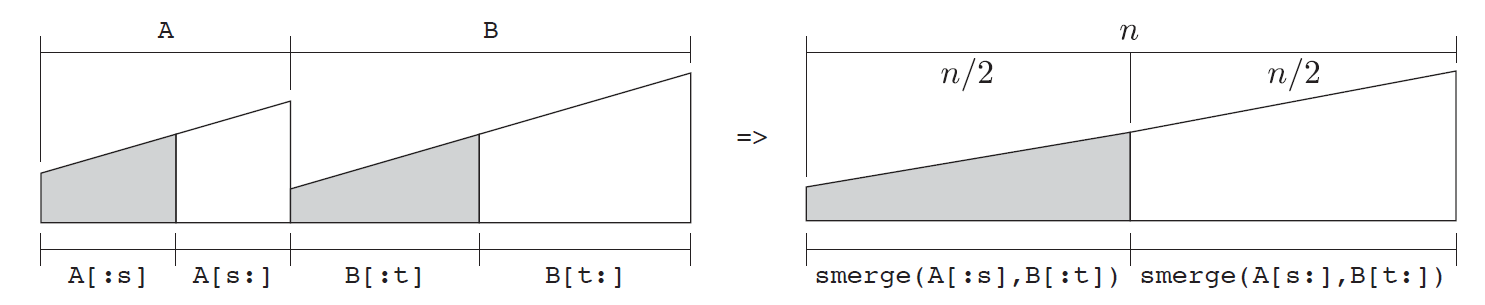
\includegraphics[width=1\linewidth]{2}
\end{figure}

\textbf{Step 1:} Find indices $s$ and $t$ such that $s+t=\dfrac{n}{2}$ and prefix subarrays \texttt{A[:s]} and \texttt{B[:t]} together contain the smallest $\dfrac{n}{2}$ keys from $A$ and $B$ combined.
 
\textbf{Step 2:} Recursively compute \texttt{X = smerge(A[:s], B[:t])} and \texttt{Y = smerge(A[s:], B[t:])}, and return their concatenation \texttt{X + Y}, a sorted array consisting of all items from $A$ and $B$.
 
 For example, if $A=[1,3,4,6,8]$ and $B=[2,5,7]$, we find $s=3$ and $t=1$ and then recursively compute:
 
 \centerline{\texttt{smerge([1,3,4], [2]) + smerge([6,8], [5,7]) = [1,2,3,4] + [5,6,7,8]}}
 
 (1) Describe an algorithm to find indices $s$ and $t$ satisfying step (1) in $O(n)$ time, using only $O(1)$ additional space beyond array $A$ and $B$ themselves. Remember to argue the correctness and running time of your algorithm.
\par\textbf{Solution:}
\par Create two pointers pointing to the first entries of the two arrays respectively, initialize both $s$ and $t$ to zero. Each time compare two values of these pointed values, increase $s$ and move the pointer of $A$ to the next entry if the value in $A$ which is pointed is smaller, increase $t$ and move the pointer of $B$  to the next entry if the value in $B$ which is pointed is smaller. Iterate until $s + t == \frac{n}{2}$.
\par The next smallest value of $A$ and $B$ combined can be found between the smallest values of remaining entries of $A$ and $B$ respectively. Since the two arrays $A$ and $B$ are already sorted, the smallest values of remaining entries of $A$ and $B$ are the first entries of $A$ and $B$ respectively, so comparing these two entries can get the next smallest value. Since $s$ and $t$ are increased within that process, $s$ and $t$ always indicates the numbers of smallest values chosen from $A$ and $B$ respectively.
\par In each iteration, the time for increase $s$ or $t$ is O(1) and the time for moving the pointer is also O(1), since the whole process iterates $\frac{n}{2}$ times, thus the total time is $O(n)$.
 
\pagebreak

(2) Write and solve a recurrence for $T(n)$, the running time of \texttt{smerge(A,B)} when $A$ and $B$ contain a total of $n$ items. Please show your steps. How does this running time compare to the \texttt{merge} step of \texttt{MergeSort()}?
\par\textbf{Solution:}
\par Since \texttt{smerge} needs to find $s$ and $t$ in $O(n)$, then invoke another two \texttt{smerge}s, the recurrence relation is:
\begin{align*}
	T(n)\ =\ 2T(\frac{n}{2})\ +\ O(n),\ T(2)\ =\ O(1)
\end{align*}
\par The recurrence tree is shown as follow:

\begin{tikzpicture}[level/.style={sibling distance=65mm/#1}]
\node [circle,draw] (z){$T(n)$}
  child {node [circle,draw] (a) {$T(\frac{n}{2})$}
    child {node [circle,draw] (b) {$T(\frac{n}{2^2})$}
      child {node {$\vdots$}
        child {node [circle,draw] (d) {($T\frac{n}{2^k})$}}
        child {node [circle,draw] (e) {$T(\frac{n}{2^k})$}}
      } 
      child {node {$\vdots$}}
    }
    child {node [circle,draw] (g) {$T(\frac{n}{2^2})$}
      child {node {$\vdots$}}
      child {node {$\vdots$}}
    }
  }
  child {node [circle,draw] (j) {$T(\frac{n}{2})$}
    child {node [circle,draw] (k) {$T(\frac{n}{2^2})$}
      child {node {$\vdots$}}
      child {node {$\vdots$}}
    }
  child {node [circle,draw] (l) {$T(\frac{n}{2^2})$}
    child {node {$\vdots$}}
    child {node (c){$\vdots$}
      child {node [circle,draw] (o) {$T(\frac{n}{2^k})$}}
      child {node [circle,draw] (p) {$T(\frac{n}{2^k})$}
        child [grow=right] {node (q) {$=$} edge from parent[draw=none]
          child [grow=right] {node (q) {\qquad $O_{k = \lg_2 n-1}(k\cdot\frac{n}{k})$} edge from parent[draw=none]
            child [grow=up] {node (r) {$\vdots$} edge from parent[draw=none]
              child [grow=up] {node (s) {$O(4\cdot\frac{n}{4})$} edge from parent[draw=none]
                child [grow=up] {node (t) {$O(2\cdot\frac{n}{2})$} edge from parent[draw=none]
                  child [grow=up] {node (u) {$O(n)$} edge from parent[draw=none]}
                }
              }
            }
            child [grow=down] {node (v) {$O(n\cdot \lg n)$}edge from parent[draw=none]}
          }
        }
      }
    }
  }
};
\path (a) -- (j) node [midway] {+};
\path (b) -- (g) node [midway] {+};
\path (k) -- (l) node [midway] {+};
\path (k) -- (g) node [midway] {+};
\path (d) -- (e) node [midway] {+};
\path (o) -- (p) node [midway] {+};
\path (o) -- (e) node (x) [midway] {$\cdots$}
  child [grow=down] {
    node (y) {}
    edge from parent[draw=none]
  };
\path (q) -- (r) node [midway] {+};
\path (s) -- (r) node [midway] {+};
\path (s) -- (t) node [midway] {+};
\path (s) -- (l) node [midway] {=};
\path (t) -- (u) node [midway] {+};
\path (z) -- (u) node [midway] {=};
\path (j) -- (t) node [midway] {=};
\path (y) -- (x) node [midway] {};
\path (v) -- (y)
  node (w) [midway] {};
\path (q) -- (v) node [midway] {=};
\path (e) -- (x) node [midway] {+};
\path (o) -- (x) node [midway] {+};
\path (y) -- (w) node [midway] {};
\path (v) -- (w) node [midway] {};
\path (r) -- (c) node [midway] {$\cdots$};
\end{tikzpicture}

\par The runtime of \texttt{smerge} is $O(n\cdot \lg n)$, which is larger than the asymptotic runtime of \texttt{merge}.

\vspace{2em}

(3) Let \texttt{smerge\_sort(A)} be a variant of \texttt{MergeSort(A)} that uses \texttt{smerge} in place of \texttt{merge}. Write and solve a recurrence for the running time of \texttt{smerge\_sort(A)}. Please show your steps.
\par\textbf{Solution:}
\par The recurrence relation is:
\begin{align*}
	T(n)\ =\ 2T(\frac{n}{2})\ +\ O(n\cdot \lg n),\ T(1) = O(1)
\end{align*}
\par The recurrence tree is shown as follow:

\begin{tikzpicture}[level/.style={sibling distance=63mm/#1}]
\node [circle,draw] (z){$T(n)$}
  child {node [circle,draw] (a) {$T(\frac{n}{2})$}
    child {node [circle,draw] (b) {$T(\frac{n}{2^2})$}
      child {node {$\vdots$}
        child {node [circle,draw] (d) {($T\frac{n}{2^k})$}}
        child {node [circle,draw] (e) {$T(\frac{n}{2^k})$}}
      } 
      child {node {$\vdots$}}
    }
    child {node [circle,draw] (g) {$T(\frac{n}{2^2})$}
      child {node {$\vdots$}}
      child {node {$\vdots$}}
    }
  }
  child {node [circle,draw] (j) {$T(\frac{n}{2})$}
    child {node [circle,draw] (k) {$T(\frac{n}{2^2})$}
      child {node {$\vdots$}}
      child {node {$\vdots$}}
    }
  child {node [circle,draw] (l) {$T(\frac{n}{2^2})$}
    child {node {$\vdots$}}
    child {node (c){$\vdots$}
      child {node [circle,draw] (o) {$T(\frac{n}{2^k})$}}
      child {node [circle,draw] (p) {$T(\frac{n}{2^k})$}
        child [grow=right] {node (q) {$=$} edge from parent[draw=none]
          child [grow=right] {node (q) {\quad\qquad $O_{k = \lg n}(k\cdot\frac{n}{k}\cdot \lg {\frac{n}{k}})$} edge from parent[draw=none]
            child [grow=up] {node (r) {$\vdots$} edge from parent[draw=none]
              child [grow=up] {node (s) {$O(4\cdot\frac{n}{4}\cdot \lg {\frac{n}{4}})$} edge from parent[draw=none]
                child [grow=up] {node (t) {$O(2\cdot\frac{n}{2}\cdot \lg {\frac{n}{2}})$} edge from parent[draw=none]
                  child [grow=up] {node (u) {$O(n\cdot \lg n)$} edge from parent[draw=none]}
                }
              }
            }
            child [grow=down] {node (v) {$O(n\cdot \lg^2 n)$}edge from parent[draw=none]}
          }
        }
      }
    }
  }
};
\path (a) -- (j) node [midway] {+};
\path (b) -- (g) node [midway] {+};
\path (k) -- (l) node [midway] {+};
\path (k) -- (g) node [midway] {+};
\path (d) -- (e) node [midway] {+};
\path (o) -- (p) node [midway] {+};
\path (o) -- (e) node (x) [midway] {$\cdots$}
  child [grow=down] {
    node (y) {}
    edge from parent[draw=none]
  };
\path (q) -- (r) node [midway] {+};
\path (s) -- (r) node [midway] {+};
\path (s) -- (t) node [midway] {+};
\path (s) -- (l) node [midway] {=};
\path (t) -- (u) node [midway] {+};
\path (z) -- (u) node [midway] {=};
\path (j) -- (t) node [midway] {=};
\path (y) -- (x) node [midway] {};
\path (v) -- (y)
  node (w) [midway] {};
\path (q) -- (v) node [midway] {=};
\path (e) -- (x) node [midway] {+};
\path (o) -- (x) node [midway] {+};
\path (y) -- (w) node [midway] {};
\path (v) -- (w) node [midway] {};
\path (r) -- (c) node [midway] {$\cdots$};
\end{tikzpicture}

\par Thus the runtime complexity of \texttt{smerge\_sort} is $O(n\cdot \lg^2 n)$.

\end{document}